\documentclass[dvipdfmx,12pt]{beamer}
\usepackage{newtxtext,newtxmath}
\usepackage{lipsum}
\usetheme{CambridgeUS}
\usepackage{bxdpx-beamer}
\usepackage{pxjahyper}
\usepackage{minijs}
\usepackage{mathpazo}
\usepackage{amsmath,amssymb}
\usepackage{graphicx}
\usepackage{array}
\usepackage{tikz}
\usepackage{wrapfig}
\usepackage{float}
\usepackage{here}
\usepackage{lscape}
\setbeamertemplate{navigation symbols}{}

\title{Reference Dependence and \\ Monetary Incentive}
\subtitle{-Evidence from Major League Baseball-}
\author{Reio TANJI\footnote{ot.shunie.rt@gmail.com} }
\date{Mar. 5th, 2019}
\institute{Osaka University, Graduate Scool of Economics}

\begin{document}

\begin{frame}\frametitle{}
  \titlepage
\end{frame}

\section*{Table of Contents}
\begin{frame}\frametitle{Contents}
  \tableofcontents
\end{frame}

\section{Introduction}

\begin{frame}\frametitle{Abstract}
  \begin{itemize}
    \item This paper explored the relationship between observed reference dependent behavior and monetary incentives.

    \item Specifically, this paper used performance stats and contract design of Major League Baseball (MLB) players, and identified their salary determination procedure.

    \item MLB players have round-number reference dependence about their performance indexes, which is not caused by their monetary incentives.

  \end{itemize}
\end{frame}

\begin{frame}\frametitle{Literature}
  \begin{itemize}
    \item There are researches that use cases from athletes' decision making.
  \end{itemize}

    \begin{block}{Reference Dependence of Athletes}
      \begin{itemize}
        \small
        \item Pope and Schweizer (2011, AER) pointed out that for the professional golf players regard ``par'' as a reference point, which results in the different probability of success in their putts.

        \item Allen et al. (2016) identified existance of reference point dependence of marathon runners, using data about the finish time of enormous number of races in the United States.

        $\Rightarrow$ Runners try to goal before the round numbers, and it results in observed excess mass, or ``bunching'' around 4 hours.

      \end{itemize}
    \end{block}
\end{frame}

\begin{frame}\frametitle{Literature}
  \begin{itemize}
    \item Pope and Simonsohn (2011) picked up the case of Major League Baseball (MLB) players about the observed attitude to their performance indexes.

    \item MLB position players make effort to manipulate their batting-average (AVG), in order to meet their internal goals: .300

    \item As a result, there is observed excess mass, or ``bunching'' around .300 of AVG.
  \end{itemize}
  \begin{figure}
    \small
    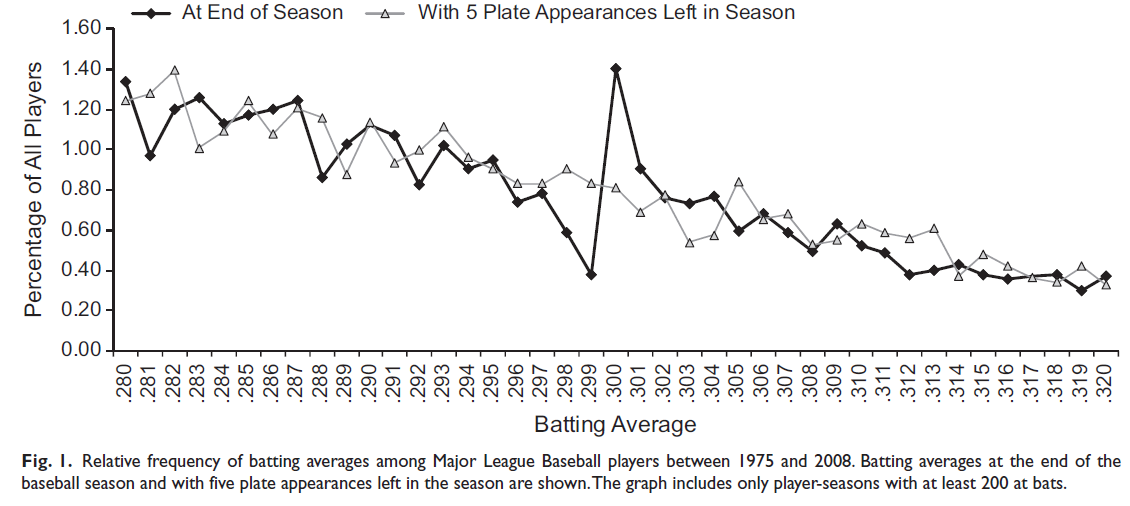
\includegraphics[keepaspectratio, scale = 0.33]{graphs/PS_fig1}
    \caption{Excess Mass Around .300 (quated from Pope and Simonsohn (2011))}
    \label{PS_fig}
  \end{figure}
\end{frame}

\begin{frame}\frametitle{Contribution}
  \begin{itemize}
    \item The case of MLB is different from that of marathon in that players are professinal, and receive salary, or monetary rewards.

    \item There may exist an economically reasonable factor that leads them to bunching.

    --The fact that a player achieves round-number of a performance index (such as .300 of batting-average) itself is to be rewarded

    \item The contribution of our research is to explore this: examine if there exists any monetary incentives that make players make effort to the cutoff point.
  \end{itemize}
\end{frame}

\section{Methodology and Data}
\begin{frame}\frametitle{Flow of Identification}
  \begin{enumerate}
    \item First, we follow Pope and Simonsohn (2011):

    identify bunching around round-numbers of various indexes.

    -- We test not only batting-average, but also other indexes of position player.

    \item Then, we test if there exists additional monetary bonus where bunching was observed.
  \end{enumerate}
  \begin{center}
    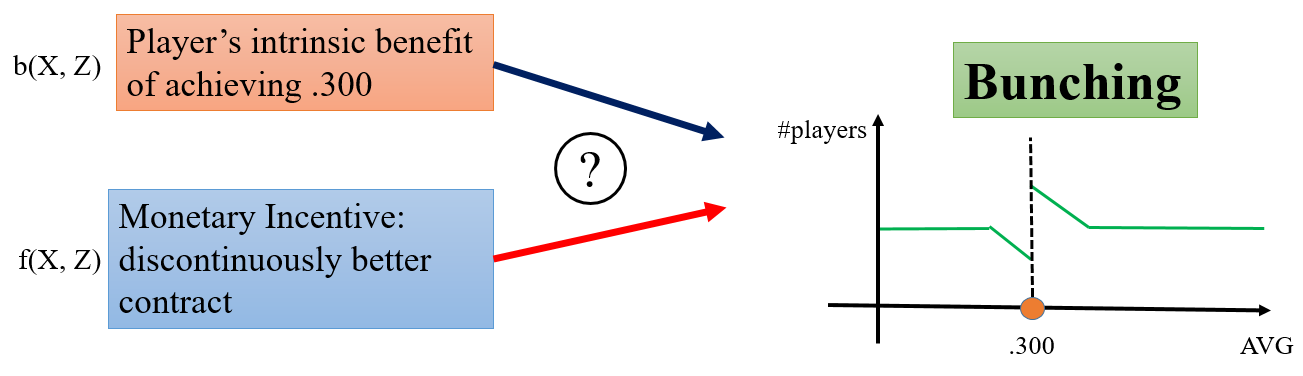
\includegraphics[keepaspectratio, scale=0.5]{output/bunching_visualize_3.png}
  \end{center}
\end{frame}

\begin{frame}\frametitle{Identification of Bunching}
  \begin{tabular}{lr}
    \begin{minipage}[H]{0.45\textwidth}
      \small
      \begin{itemize}
        \item We exploit the McCrary (2007)'s manipulation test, which is used in regression discontinuity design.

        \item Make local approximation of the histgram of the variable of interest, and calculate the predicted values of $f(r)$ at the cutoff point, from both above and below there.
      \end{itemize}
    \end{minipage}
    &
    \begin{minipage}[H]{0.5\textwidth}
      \begin{figure}
        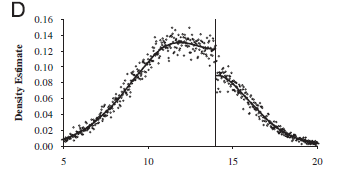
\includegraphics[keepaspectratio, scale = 0.8]{graphs/McCrary_figD.png}
        \caption{Discontinuous frequency (quated from McCrary(2007))}
        \label{McC}
      \end{figure}
    \end{minipage}
  \end{tabular}
\end{frame}

\begin{frame}\frametitle{Identification of Reward Function}
  \begin{itemize}
    \small
    \item Contract design is estimated by following local-linear regression:
    \begin{align*}
      \footnotesize
      w_{it} = \beta_0 + \beta_1 \text{PERF}_{it} + &\beta_2 \text{ABOVE}_{it} + \beta_3 \text{PERF}_{it} \times \text{ABOVE}_{it} \\
      \text{where} \\
      w_{it}: & \text{ log salary of the next season} \\
      \text{PERF}_{it}: & \text{ performance index} \\
      \text{ABOVE}_{it}: & \text{ indicator for achievement}
    \end{align*}

    We also conduct analysis including other performance and other player specific charactaristics.
  \end{itemize}
\end{frame}

\begin{frame}\frametitle{Data Description}
  We obtain information about the players' stats (indexes) and annual salary.
  \begin{itemize}
    \item Stats Data
    \begin{itemize}
      \item From \textit{FanGraphs}

      \item Play stats from 1957 to 2018

      \item We restrict the sample to the players with at least 200 plate-appearances $N=18143$ (62 seasons $\times$ players)
    \end{itemize}
  \end{itemize}
  \begin{center}
    \includegraphics[keepaspectratio, scale=.25]{output/FanGraphs_2.png}
  \end{center}
\end{frame}

\begin{frame}
  \begin{itemize}
    \item Salary Data
    \begin{itemize}
      \item From \textit{USA TODAY} and \textit{Baseball References}

      \item Contract information from 1987 to 2017 $N=8915$(31 seasons $\times$ players)
      \begin{itemize}
        \item Fixed part of the salary of each player

        \item Information about possession of free agency, the right to negotiate any team in MLB.
      \end{itemize}
    \end{itemize}
  \end{itemize}
  \begin{center}
    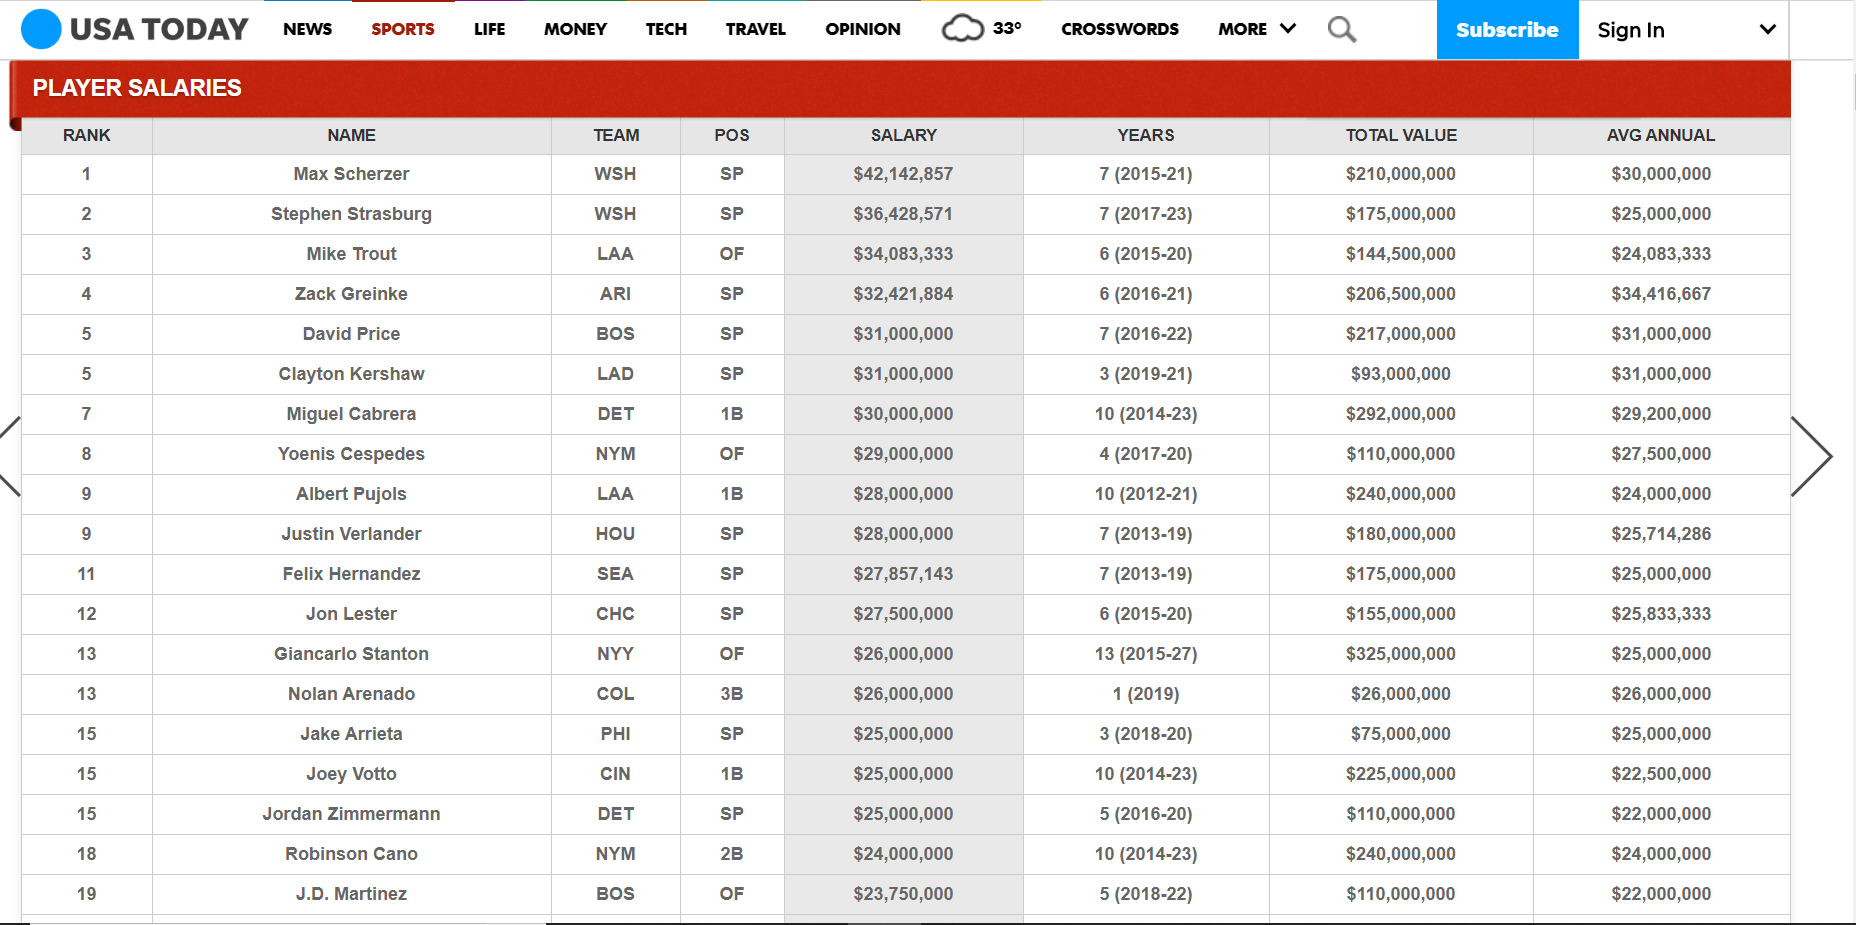
\includegraphics[keepaspectratio, scale=.3]{output/USATODAY_2.png}
  \end{center}
\end{frame}

\section{Results}

\begin{frame}\frametitle{Results}
  \large
  Step 1. Bunching
\end{frame}

\begin{frame}\frametitle{Bunching: McCrary's Test}
  \begin{figure}
    \centering
    \caption{Histgram of Batting-Average}        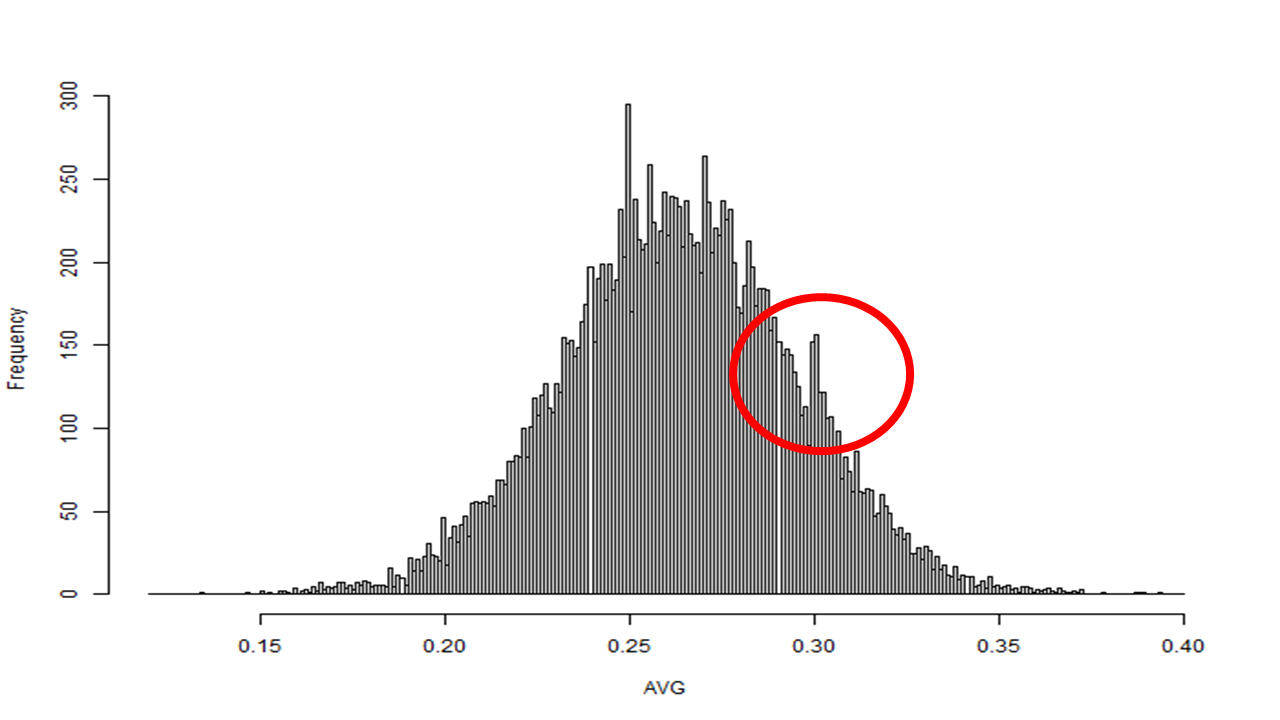
\includegraphics[width=10cm, height=7cm, angle=0]{graphs/hist_AVG_all_withO.png}
    \label{AVG_Histgram}
  \end{figure}
\end{frame}


\begin{frame}
  \begin{table}
    \tiny
    \centering
    \caption{Test for Bunching, leastPA $= 200$}
    \begin{tabular}{lcccccc}\hline
      index & type & cutpoint & binsize & bandwidth & $\theta$ & $z$
      \\ \hline \hline
      AVG & rate & .300 & .001 & .019 &  .499 & 7.442*** \\
      & & & & & (.067) & \\
      & & .250 & .001 & .024 & .212 & 5.061*** \\
      & & & & & (.042) & \\
      OBP & rate & .350 & .001 & .024 &  .139 & 2.854** \\
      & & & & & (.049) &  \\
      HR & cumulative & 20 & 1 & 5.309 & .259 & 3.465*** \\
      & & & & & (.075)  & \\
      RBI & cumulative & 100 & 4 & 15.423 & .311 & 3.295*** \\
      & & & & & (.094) & \\
      SB & cumulative & 30 & 1 & 10.000 & .529 & 4.274*** \\
      & & & & & (.124) & \\
      & & 40 & 1 & 11.505 & .481 & 2.764** \\
      & & & & & (.174) & \\
      PA & cumulative & 500 & 1 & .003 & .160 & 2.515* \\
      & & & & &(.063) & \\
      H & cumulative & 200 & 1 & 18.922 & .453 & 2.547 * \\
      & & & & & (.178) & \\ \hline \hline
      Note & \multicolumn{6}{r}{
      ***: $p<0.1\%$, **: $p<1\%$, *: $p<5\%$.
      }\\
      \multicolumn{7}{r}{
      Bandwidth is optimized following the method of McCrary(2008).
      }
    \end{tabular}
    \label{Bunch-True}
  \end{table}
\end{frame}

\begin{frame}\frametitle{Results}
  \large
  Step 2. Monetary Incentive
\end{frame}

\begin{frame}\frametitle{}
  
% Table created by stargazer v.5.2.2 by Marek Hlavac, Harvard University. E-mail: hlavac at fas.harvard.edu
% Date and time: ��, 12 13, 2018 - 15:22:37
\begin{table}[H] \centering
  \caption{Regression on Log-Salary, Including Interaction Term: around .300}
  \label{AVG300_A}
\fontsize{5pt}{4pt}\selectfont
\begin{tabular}{@{\extracolsep{-15pt}}lcccccc}
\\[-1.8ex]\hline
\hline \\[-1.8ex]
 & \multicolumn{6}{c}{\textit{Dependent variable:}} \\
\cline{2-7}
\\[-1.8ex] & \multicolumn{6}{c}{Loggarithm of Salary Next Year} \\
\\[-1.8ex] & \multicolumn{4}{c}{\textit{OLS}} & \multicolumn{2}{c}{\textit{felm}} \\
\\[-1.8ex] & (1) & (2) & (3) & (4) & (5) & (6)\\
\hline \\[-1.8ex]
 Constant & 11.166$^{***}$ & $-$6.616$^{***}$ & $-$5.203$^{***}$ & $-$5.319$^{***}$ &  &  \\
  & (.423) & (.665) & (.671) & (.667) &  &  \\
  & & & & & & \\
 AVG & 11.513$^{***}$ & 11.620$^{***}$ & 4.361$^{***}$ & 4.221$^{***}$ & 3.774$^{**}$ & 3.808$^{**}$ \\
  & (1.537) & (1.209) & (1.209) & (1.201) & (1.194) & (1.189) \\
  & & & & & & \\
 AVG\_300 & $-$.169 & $-$.413 & $-$.191 & $-$.142 & $-$.287 & $-$.069 \\
  & (1.050) & (.821) & (.785) & (.780) & (.775) & (.706) \\
  & & & & & & \\
  AVG:AVG\_300 & .663 & 1.428 & .681 & .540 & .996 & .160 \\
  & (3.429) & (2.681) & (2.566) & (2.549) & (2.532) & (2.312) \\
  & & & & & & \\
 FLD &  & .006$^{***}$ & .008$^{***}$ & .007$^{***}$ & .007$^{***}$ & .008$^{***}$ \\
  &  & (.002) & (.002) & (.002) & (.002) & (.002) \\
  & & & & & & \\
 BsR &  & .009$^{*}$ & .002 & .003 & .004 & .020$^{***}$ \\
  &  & (.005) & (.005) & (.005) & (.004) & (.005) \\
  & & & & & & \\
\hline \\[-1.8ex]
Season dummies &  & X & X & X & X & X \\
WPA & & & X & X & X & X  \\
AGE (quadratic) &  & X & X & X & X &  \\
FA dummy &  &  &  & X & X & X \\
Position dummies &  &  & X & X &  &  \\
Fixed effects &  &  &  &  & Team & Individual \\
Observations & 5,960 & 5,930 & 5,930 & 5,930 & 5,930 & 5,930 \\
R$^{2}$ & .035 & .420 & .470 & .478 & .488 & .744 \\
Adjusted R$^{2}$ & .035 & .416 & .466 & .473 & .482 & .660 \\
Residual Std. Error & 1.286 (df = 5956) & 1.001 (df = 5892) & .957 (df = 5881) & .950 (df = 5880) & .943 (df = 5860) & .764 (df = 4459) \\
F Statistic & 71.983$^{***}$ (df = 3; 5956) & 115.152$^{***}$ (df = 37; 5892) & 108.865$^{***}$ (df = 48; 5881) & 109.753$^{***}$ (df = 49; 5880) &  &  \\
\hline
\hline \\[-1.8ex]
\textit{Note:}  & \multicolumn{6}{r}{$^{*}$p$<$0.05; $^{**}$p$<$0.01; $^{***}$p$<$0.001} \\
& \multicolumn{6}{r}{The bandwidth is same as RDD for .300 of AVG.} \\
& \multicolumn{6}{r}{FLD and BsR stands for the contribution of the player to the team, expressed by the runs they earned.} \\
& \multicolumn{6}{r}{WPA is ``win-percentage added.''} \\
& \multicolumn{6}{r}{FA dummy indicates the possession of the free agency.}\\
& \multicolumn{6}{r}{":" stands for the interaction term of the two elements.} \\
\end{tabular}
\end{table}

\end{frame}


\section{Conclusion}

\begin{frame}\frametitle{Conclusion}
  Main Findings
  \begin{enumerate}
    \item Bunching is observed in their performance indexes, caused by the players' adjustment of their effort level to meet them with some round numbers.

    \item There exist no monetary incentives in their contracts that makes players to do so.

  \end{enumerate}

  \begin{itemize}
    \item Robustness checks do not change the results.

    \item Because of data limitations, we could not test the

  \end{itemize}

\end{frame}

\section*{References}

\begin{frame}\frametitle{References}
  \tiny
  \begin{thebibliography}{99}
    \bibitem PPope and Simonsohn. 2011.
    Round Numbers as Goals: Evidence From Baseball, SAT Takers, and the Lab
    \textit{Psychological Science} 22(1) 7179

    \bibitem HHakes and Sauer. 2006.
    An Economic Evaluation of the Moneyball Hypothesis
    \textit{Journal of Economic Perspectives} Volume 20, Number 3 - Summer 2006 - Pages 173185

    \bibitem AAllen, Dechow, Pope and Wu. 2016.
    Reference-Dependent Preferences: Evidence from Marathon Runners \textit{Management Science} 63(6):1657-1672.

    \bibitem PPope and Schweizer. 2011.
    Is Tiger Woods Loss Averse? Persistent Bias in the Face of Experience, Competition, and High Stakes
    \textit{American Economic Review} 101 (February 2011): 129157

    \bibitem{}Kahneman and Tversky. 1979.
    Prospect Theory: An Analysis of Decision under Risk.
    \textit{Econometrica}
    Journal of the Econometric Society47 (2):263291.

    \bibitem{}McCrary. 2007.
    Manipulation of the running variable in the regression discontinuity design: A density test
    \textit{Journal of Econometrics} 142 (2008) 698 - 714

    \bibitem{}Krautmann and Oppenheimer. 2002.
    Contract Length and the Return to Performance in Major League Baseball
    \textit{Journal of Sports Economics} February 2002

    \bibitem{}Tversky and Kahneman. 1992.
    Advances in Prospect Theory: Cumulative Representation of Uncertainty
    \textit{Journal of Risk and Uncertainty}, 5:297 - 323 (1992)

    \bibitem{}Imbens and Kalyanaraman. 2009.
    \textit{NBER Working Paper Series.} 14726

    \bibitem{}Alex Rees-Jones. 2018.
    Quantifying Loss-Averse Tax Manipulation
    \textit{Review of Economic Studies} (2018) 85, 1251 - 1278
  \end{thebibliography}
\end{frame}

\begin{frame}\frametitle{Data}
  \begin{itemize}
    \item \textit{Fangraphs Baseball}

    https://www.fangraphs.com/

    \item \textit{Baseball Reference}

    https://www.baseball-reference.com

    \item \textit{USA TODAY}

    https://www.usatoday.com/sports/mlb/

    \item \textit{Baseball Prospectus: Cot's Baseball Contracts}

    https://www.baseballprospectus.com/
  \end{itemize}
\end{frame}

\section*{Appendix}
\begin{frame}\frametitle{Appendix}
  \large
  \begin{itemize}

    \item Robustness

    \item Alternative Interpretations

    \item Extention
  \end{itemize}
\end{frame}

\section*{Robustness}

\begin{frame}\frametitle{Plural-Year Contract}
  \begin{itemize}
    \item If players agree plural-year contracts, then achieving the reference points are not reflected to their rewards immediately.

    \item We restrict the samples to those who have the right of free agency: those who agreed a new contract with their team.
  \end{itemize}
\end{frame}

\begin{frame}
  
% Table created by stargazer v.5.2.2 by Marek Hlavac, Harvard University. E-mail: hlavac at fas.harvard.edu
% Date and time: ��, 12 24, 2018 - 22:35:23
\begin{table}[H] \centering
  \caption{Regression on Log-Salary: around .300, Including Only FA Players}
  \label{AVG300_F}
\fontsize{5pt}{4pt}\selectfont
\begin{tabular}{@{\extracolsep{-15pt}}lcccccc}
\\[-1.8ex]\hline
\hline \\[-1.8ex]
 & \multicolumn{6}{c}{\textit{Dependent variable:}} \\
\cline{2-7}
\\[-1.8ex] & \multicolumn{6}{c}{Loggarithm of Salary Next Year} \\
\\[-1.8ex] & \multicolumn{4}{c}{\textit{OLS}} & \multicolumn{2}{c}{\textit{felm}} \\
\\[-1.8ex] & (1) & (2) & (3) & (4) & (5) & (6)\\
\hline \\[-1.8ex]
 Constant & 7.033$^{**}$ & 7.339$^{*}$ & 7.114$^{*}$ & 7.524$^{*}$ &  &  \\
  & (2.374) & (3.225) & (3.243) & (3.062) &  &  \\
  & & & & & & \\
 AVG & 26.614$^{**}$ & 26.230$^{***}$ & 22.624$^{**}$ & 14.443$^{*}$ & 16.909$^{*}$ & 13.286 \\
  & (8.308) & (7.245) & (7.355) & (6.851) & (6.961) & (10.076) \\
  & & & & & & \\
 AVG\_300 & 6.740 & 2.770 & 1.883 & .969 & 1.636 & 2.727 \\
  & (4.231) & (3.707) & (3.749) & (3.453) & (3.468) & (4.444) \\
  & & & & & & \\
 FLD &  & .005 & .006 & .007 & .004 & .001 \\
  &  & (.006) & (.006) & (.005) & (.005) & (.007) \\
  & & & & & & \\
 BsR &  & .027 & .025 & .019 & .016 & $-$.013 \\
  &  & (.014) & (.015) & (.014) & (.014) & (.025) \\
  & & & & & & \\
 AVG:AVG\_300 & $-$23.155 & $-$10.065 & $-$6.893 & $-$4.015 & $-$6.451 & $-$9.953 \\
  & (14.071) & (12.333) & (12.474) & (11.489) & (11.540) & (14.911) \\
  & & & & & & \\
\hline \\[-1.8ex]
Season dummies &  & X & X & X & X & X \\
WPA &  &  &  & X & X & X \\
AGE (quadratic) &  & X & X & X & X &  \\
Position dummies &  &  & X & X &  &  \\
Fixed effects &  &  &  &  & Team & Individual \\
Observations & 503 & 493 & 493 & 493 & 493 & 493 \\
R$^{2}$ & .028 & .388 & .406 & .502 & .529 & .937 \\
Adjusted R$^{2}$ & .022 & .339 & .345 & .448 & .453 & .735 \\
Residual Std. Error & 1.052 (df = 499) & .870 (df = 455) & .866 (df = 446) & .795 (df = 444) & .791 (df = 424) & .551 (df = 117) \\
F Statistic & 4.824$^{**}$ (df = 3; 499) & 7.808$^{***}$ (df = 37; 455) & 6.630$^{***}$ (df = 46; 446) & 9.328$^{***}$ (df = 48; 444) &  &  \\
\hline
\hline \\[-1.8ex]
\textit{Note:}  & \multicolumn{6}{r}{$^{*}$p$<$0.05; $^{**}$p$<$0.01; $^{***}$p$<$0.001} \\
& \multicolumn{6}{r}{The bandwidth is same as RDD for .300 of AVG.} \\
& \multicolumn{6}{r}{FLD and BsR stands for the contribution of the player to the team, expressed by the runs they earned.} \\
& \multicolumn{6}{r}{WPA is ``win-percentage added.''} \\
& \multicolumn{6}{r}{FA dummy indicates the possession of the free agency.}\\
& \multicolumn{6}{r}{":" stands for the interaction term of the two elements.} \\
\end{tabular}
\end{table}

\end{frame}

\begin{frame}\frametitle{Downward Biases}
  \begin{itemize}
    \item Players can ``manipulate'' their batting-average by stopping to appear to the plate after reaching .300 of batting-average (Pope and Simonsohn, 2011).

    \item If team managers can detect such players, then managers offer them contracts that is offered to the players with .299.

    $\Rightarrow$ the estimated size of notch or kink were likely to be underestimated.

    \item To deal with this problem, we remove the samples around .300, and made the same regression.
  \end{itemize}
\end{frame}

\begin{frame}
  
% Table created by stargazer v.5.2.2 by Marek Hlavac, Harvard University. E-mail: hlavac at fas.harvard.edu
% Date and time: ��, 12 24, 2018 - 22:35:20
\begin{table}[H] \centering
  \caption{Without Players around the Cutoff}
  \label{AVG300_E}
\fontsize{5pt}{4pt}\selectfont
\begin{tabular}{@{\extracolsep{-15pt}}lcccccc}
\\[-1.8ex]\hline
\hline \\[-1.8ex]
 & \multicolumn{6}{c}{\textit{Dependent variable:}} \\
\cline{2-7}
\\[-1.8ex] & \multicolumn{6}{c}{Loggarithm of Salary Next Year} \\
\\[-1.8ex] & \multicolumn{4}{c}{\textit{OLS}} & \multicolumn{2}{c}{\textit{felm}} \\
\\[-1.8ex] & (1) & (2) & (3) & (4) & (5) & (6)\\
\hline \\[-1.8ex]
 Constant & 11.457$^{***}$ & $-$6.672$^{***}$ & $-$5.567$^{***}$ & $-$5.734$^{***}$ &  &  \\
  & (.465) & (.709) & (.716) & (.711) &  &  \\
  & & & & & & \\
 AVG & 10.428$^{***}$ & 11.419$^{***}$ & 4.782$^{***}$ & 4.643$^{***}$ & 4.346$^{***}$ & 4.393$^{***}$ \\
  & (1.697) & (1.328) & (1.325) & (1.315) & (1.306) & (1.333) \\
  & & & & & & \\
 AVG\_300 & $-$1.277 & $-$.032 & .274 & .320 & .136 & .190 \\
  & (1.440) & (1.122) & (1.076) & (1.068) & (1.062) & (.968) \\
  & & & & & & \\
  AVG:AVG\_300 & 4.263 & .309 & $-$.757 & $-$.897 & $-$.333 & $-$.657 \\
  & (4.600) & (3.582) & (3.438) & (3.412) & (3.393) & (3.103) \\
  & & & & & & \\
 FLD &  & .007$^{***}$ & .008$^{***}$ & .008$^{***}$ & .008$^{***}$ & .009$^{***}$ \\
  &  & (.002) & (.002) & (.002) & (.002) & (.002) \\
  & & & & & & \\
 BsR &  & .006 & $-$.0003 & $-$.0003 & .0004 & .018$^{**}$ \\
  &  & (.005) & (.005) & (.005) & (.005) & (.006) \\
  & & & & & & \\
\hline \\[-1.8ex]
Season dummies &  & X & X & X & X & X \\
WPA &  &  & X & X & X & X \\
AGE (quadratic) &  & X & X & X & X &  \\
FA dummy &  &  &  & X & X & X \\
Position dummies &  &  & X & X &  &  \\
Fixed effects &  &  &  &  & Team & Individual \\
Observations & 5,259 & 5,232 & 5,232 & 5,232 & 5,232 & 5,232 \\
R$^{2}$ & .034 & .425 & .473 & .481 & .492 & .752 \\
Adjusted R$^{2}$ & .034 & .421 & .468 & .476 & .485 & .657 \\
Residual Std. Error & 1.286 (df = 5255) & .996 (df = 5194) & .955 (df = 5183) & .947 (df = 5182) & .939 (df = 5162) & .767 (df = 3787) \\
F Statistic & 62.260$^{***}$ (df = 3; 5255) & 103.758$^{***}$ (df = 37; 5194) & 96.869$^{***}$ (df = 48; 5183) & 97.991$^{***}$ (df = 49; 5182) &  &  \\
\hline
\hline \\[-1.8ex]
\textit{Note:}  & \multicolumn{6}{r}{$^{*}$p$<$0.05; $^{**}$p$<$0.01; $^{***}$p$<$0.001} \\
& \multicolumn{6}{r}{The bandwidth is same as RDD for .300 of AVG.} \\
& \multicolumn{6}{r}{FLD and BsR stands for the contribution of the player to the team, expressed by the runs they earned.} \\
& \multicolumn{6}{r}{WPA is ``win-percentage added.''} \\
& \multicolumn{6}{r}{FA dummy indicates the possession of the free agency.}\\
& \multicolumn{6}{r}{":" stands for the interaction term of the two elements.} \\
\end{tabular}
\end{table}

\end{frame}


\section*{Alternative Interpretation and Discussion}

\begin{frame}\frametitle{Piece-Rate Rewards}
  \begin{itemize}
    \item Some players receive additional payments by reaching reference points, such as .300 of batting-average.

    \item From \textit{Cot's Baseball Contracts}, we obtained specific contents of players' contracts.

    \item Players receive additional performance-dependent rewards:

    Award bonus and index-dependent bonus.

    \item Few position players sign the contract with index-dependent bonus, and all of them are related to the number of attendance:

    Plate-appearances, games-attended
  \end{itemize}
\end{frame}

\begin{frame}\frametitle{Contracts}
  \begin{itemize}
    \footnotesize
    \item Ichiro Suzuki, Outfielder, 4-year contract with Seattle Marinars (2004-'07)
    \begin{itemize}
      \footnotesize
      \item signing bonus- \$6M

      \item fixed payment- 04:\$5M, 05:\$11M, 06:\$11M, 07:\$11M

      \item performance bonuses- \$1.25M in performance bonuses for plate appearances

      \begin{itemize}
        \footnotesize
        \item \$50,000 each for 400 PAs, 2004-06

        \item \$0.1M each for 500 \& 600 PAs, 2004-06

        \item \$0.1M for 400 PAs, 2007

        \item \$0.2M each for 500 \& 600 PAs, 2007
      \end{itemize}

      \item award bonuses: \$50,000 each for Gold Glove, All Star selection

      \item trade-Protection (Veto for moving the team without his acceptance):

      limited no-trade clause (may block deals to 10 clubs)

      \item Other

      \begin{itemize}
        \footnotesize
        \item housing allowance: \$28,000 in 2004, \$29,000 in 2005, \$30,000 in 2006, \$31,000 in 2007

        \item interpreter, trainer, transportation for spring \& regular season

        \item 4 annual round-trip airline tickets from Seattle to Japan
      \end{itemize}
    \end{itemize}
  \end{itemize}
\end{frame}

\begin{frame}\frametitle{Contract Length}
  \begin{itemize}
    \item Krautmann and Oppenheimer (2002) pointed out that the longer the contract duration extend, the lower return to their performance is obtained: Players show the risk-aversion.

    \begin{align*}
      \ln(SAL_{it}) = \beta_1 &+ \beta_2 PERF_{it} \\
      &+ \beta_3 (PERF_{it} * LENGTH_{it})+ \beta_4 LENGTH_{it}
    \end{align*}
    \footnotesize
    \flushright
    * The model is quoted from Krautmann and Oppenheimer (2006).

    \flushleft
    \normalsize

    \item Estimated value of $\beta_3$ was negative.

    \item Further research considering the contract length to be required.
  \end{itemize}
\end{frame}

\section*{Extention}

\begin{frame}\frametitle{By-Time Analysis}
  \begin{itemize}
    \item By-Time analysis
    \begin{itemize}
      \item Replicate the same examination, but now we devide the sample by histrical terms:
      \begin{enumerate}
        \item Before the system of free agency regulated (-1975)

        \item Before the Strike of Players Association (-1994)

        \item Before \textit{Moneyball} (Lewis) was published (-2003)

        \item Afterward (2004-)

        * Note that because we obtain the sample of contract design only after '87, we cannot conduct the second analysis for before '86.
      \end{enumerate}

      \item Hakes and Sauer (2006) aregued that after the publication of \textit{Moneyball}, team managers regard on-base percentage as more important index to measure the players' contribution to the team they belong to.

    \end{itemize}
  \end{itemize}
\end{frame}

\begin{frame}
  \begin{table}
    \centering
    \caption{Bunching Test for the Grouped Sample by Time}
    \label{Mani-Era}
    \tiny
    \begin{tabular}{lcccccc} \hline
      index, cutpoint &  & '57-'75 &'76-'94 & '95-2003 & 2004- &full sample \\ \hline \hline
      AVG, .300 & bw & .023 & .020 & .022 & .019 & .019 \\
      & $\theta$ & .573 & .566 & .310 & .403 & .499 \\
      & & (.146) & (.120) & (.130) & (.120) & (.067) \\
      & $z$ & 3.934*** & 4.732*** & 2.393* & 3.376*** & 7.442*** \\ \hline
      AVG, .250 & bw & .028 & .028 & .032 & .027 & .024 \\
      & $\theta$ & .250 & .151 & .306 & .121 & .212 \\
      & & (.080) & (.069) & (.094)& (.076) & (.042) \\
      & $z$ & 3.149** & 2.188* & 3.242** & 1.595 & 5.061*** \\ \hline
      OBP, .350 & bw & .031 & .030 & .036 & .030 & .024 \\
      & $\theta$ & .137 & .149 & -.035 & .137 & .139 \\
      & & (.089) & (.081) & (.093) & (.082) & (.049) \\
      & $z$ & 1.538 & 1.846 & -.380 & 1.672 & 2.854** \\ \hline
      HR, 20 & bw & 6.313 & 6.677 & 10.165 & 7.273 & 5.309 \\
      & $\theta$ & .222 & .214 & .145 & .315 & .259 \\
      & & (.150) & (.123) & (.129) & (.112) & (.075) \\
      & $z$ & 1.479 & 1.751 & 1.117 & 2.819** & 3.465*** \\ \hline
      Note & \multicolumn{6}{r}{
      ***: $p<0.1\%$, **: $p<1\%$, *: $p<5\%$.
      }\\
      & \multicolumn{6}{r}{
      Bandwidth is optimized following the method of McCrary(2008).
      }
    \end{tabular}
  \end{table}
\end{frame}

\begin{frame}
  \begin{table}
    \centering
    \caption{Local-Linear Regression for the Grouped Sample by Time}
    \label{RDD_Era}
    \tiny
    \begin{tabular}{lcccccc} \hline
      index, cutpoint & bw, type &  &'87-'94 & '95-2003 & 2004- &full sample \\ \hline \hline
      AVG, .300 & LATE & bw & .024 & .042 & .030 & .045 \\
      &  & Obs. & 697 & 1806 & 1872 & 5930 \\
      &  & estimate & -.034 & .064 & .066 & .034 \\
      &  & & (.137) & (.092) & (.103) & (.056) \\
      & & $z$ & -.250 & .697 & .637 & .615 \\ \hline
      AVG, .250 & LATE & bw & .036 & .043 &.075 & .048 \\
      &  & Obs. & 1482 & 1806 & 3991 & 7271 \\
      &  & estimate & .154 & .064 & .076 & .070 \\
      &  & & (.084) & (.092) & (.060) & (.052) \\
      & & $z$ & 1.825 & .697 & 1.277 & 1.340 \\ \hline
      HR, 20 & LATE & bw & 4.183 & 3.685 & 2.46 & 3.30 \\
      &  & Obs. & 341 & 371 & 475 & 1307 \\
      &  & estimate & -.255 & -.348 & .343 & -.002 \\
      &  & & (.228) & (.218) & (.264) & (.141) \\
      & & $z$ & -1.122 & -1.600 & 1.300 & -.015 \\ \hline
      OBP, .350 & LATE & bw & .031 & .025 & .027 & .045 \\
      &  & Obs. & 1098 & 1281 & 2042 & 6525 \\
      &  & estimate & .109 & -.151 & -.030 & -.013 \\
      &  & & (.106) & (.120) & (.093) & (.049) \\
      & & $z$ & 1.031 & -1.262 & -.323 & -.272 \\ \hline
      Note: & \multicolumn{6}{r}{***: $p<0.1\%$, **: $p<1\%$, *: $p<5\%$.} \\
      & \multicolumn{6}{r}{Bandwidth is optimized following the method of Imbens-Kalyanaraman.}
    \end{tabular}
  \end{table}
\end{frame}

\end{document}
